\chapter{Results}
\index{Results@\emph{Results}}%

\section{Lexical and Metrical Prominence Patterns}
\subsection{Distributions}

\begin{figure}[htbp]
\begin{center}
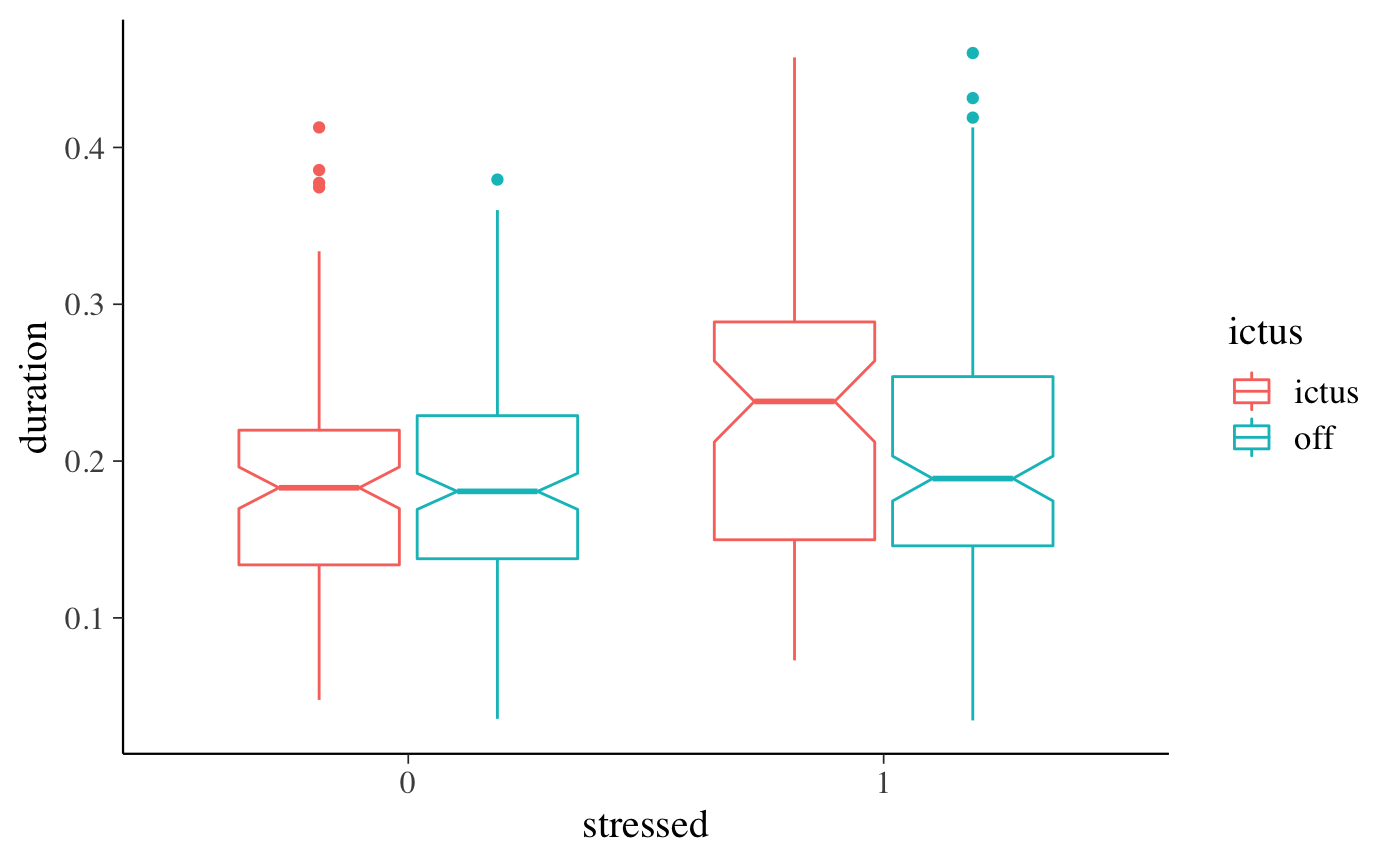
\includegraphics[width=\textwidth]{figures/strictus_box.png}
\caption{default}
\label{strickbox}
\end{center}
\end{figure}


Before analyzing the measurements, I look at the overall occurrence patterns of conflicting and concordant lexical and lyrical metrical positions. That is, do stressed syllables have a requirement or tendency to fall ``on the beat" in the song, or are they freely distributed? Likewise, do unstressed syllables tend to align with unaccented notes ``off the beat?" 


\begin{table}[ht]
\centering
\begin{tabular}{lcr}
\hline
 & un &   stressed \\
\hline
on  &   107 & 129 \\
off     &  164 & 210 \\
\hline
\end{tabular}
\label{contin}
\caption{counts of conflict(*) and concord strong-weak combinations}
\end{table}

The contingency table in \ref{contin} illustrates the counts of stressed and unstressed Estonian syllables as they fall on (ictus) and off the musical beats in the song corpus. On the beat, in ictus position, both stressed and unstressed syllables occur, and Chi-squared test finds no significant difference. Thus, both stressed and unstressed syllables may occupy the ictus "on beat" note positions in a measure. A similar pattern is seen in note positions that are off the beat, with both stressed an unstressed syllables given equal opportunity to fall in note positions that are off the beat. 

This suggests that word-level and song-level rhythmic prominence are able to act independently of each other: that is, one cannot predict from beat position in the song the stressed status of the syllable, or vice a versa. 
a chi-squared test on the contingency table using the scipy library in python \citep{2020SciPy-NMeth, mckinney-proc-scipy-2010}\footnote{\citep{reback2020pandas} can be found at \url{https://github.com/sally-ran-some} \citep{Kluyver2016jupyter}}


In \ref{chicont}, we see that there is no significant (p=0.78) tendency for stress to align with ictus or not,  and the expected values are very close to the actual value counts in \ref{chipredict}.


\begin{table}[htb]
\caption{chi-squared of stress-ictus contingency table}
\begin{center}
\begin{tabular}{ll}
\hline
chi-stat & 0.077 \\
p-value &  0.78 \\
\hline
\end{tabular}
\end{center}
\label{chicont}
\end{table}%


\begin{table}{htb}
\caption{expected values predicted from chi-squared}
\centering
\begin{tabular}{lll}
\hline
 				& un 		&   stressed \\
\hline
on	& 166 	& 207 \\
off   				&   104	 & 131 \\
\hline
\end{tabular}
\label{chipredict}
\end{table}



\subsection{Vowel Duration: song \& word stress} 
To examine the overall effects of stress and ictus on vowel duration, I exclude Q3 syllables, as they always fall in stressed position in native Estonian words.\footnote{Vowel durations for Q3 falling on and off the beat are included in appendix C} 

Using the \citep{goodrichRstanarmBayesianApplied2020} Stan extension package for R, I first construct a design-based Bayesian heirarchical regression model following \cite{heirarchyOne}. 

\begin{equation}
duration ~ stress + ictus + stress*ictus + (1|singer)
\end{equation} 
However, upon looking at the posterior distributions, it was clear there was a pattern not being explained by the model. The random intercept for singer had been chosen based on the assumption that singers would vary from each other. However, as you can see in \ref{scatterSongs}, there are distinct groupings that may instead correspond to each song. The singer as random intercept notion had been based on phonetics research in natural speech, however, in this case the song was the best random intercept to include in the model for vowel duration. Performers tend to be consistent compared with each other in songs, while songs with differing speeds (beats per minute) are better predictors for vowel duration. Thus, the (ad hoc) model I will focus on for this analysis is as follows: 

\begin{equation}
duration ~ stress + ictus + stress*ictus + (1|song)
\end{equation}

In \ref{durStrictus} is the summary of posterior statistics. 
% latex table generated in R 4.1.2 by xtable 1.8-4 package
% Thu Aug 18 16:51:21 2022
\begin{longtable}{lrrrrrrrrrr}
  \toprule
Parameter & Rhat & n\_eff & mean & sd & se\_mean & 2.5\% & 25\% & 50\% & 75\% & 97.5\% \\ 
  \midrule
Intercept & 1.004 &  963 & 0.190 & 0.024 & 0.001 & 0.142 & 0.174 & 0.190 & 0.205 & 0.234 \\ 
  ictusoff & 1.000 & 3073 & 0.004 & 0.010 & 0.000 & -0.014 & -0.002 & 0.004 & 0.011 & 0.023 \\ 
  stressed1 & 1.000 & 2791 & 0.041 & 0.012 & 0.000 & 0.016 & 0.032 & 0.041 & 0.049 & 0.064 \\ 
  quantity2 & 1.000 & 3076 & -0.038 & 0.012 & 0.000 & -0.061 & -0.047 & -0.039 & -0.030 & -0.016 \\ 
  ictusoff:stressed1 & 1.000 & 3494 & -0.018 & 0.013 & 0.000 & -0.042 & -0.026 & -0.018 & -0.009 & 0.006 \\ 
  stressed1:quantity2 & 1.000 & 3166 & 0.029 & 0.013 & 0.000 & 0.005 & 0.021 & 0.029 & 0.038 & 0.054 \\ 
  ictusoff:quantity2 & 1.000 & 2818 & -0.002 & 0.013 & 0.000 & -0.027 & -0.010 & -0.001 & 0.007 & 0.023 \\ 
  b[(Intercept) song:9] & 1.003 & 1022 & 0.088 & 0.025 & 0.001 & 0.039 & 0.072 & 0.087 & 0.104 & 0.136 \\ 
  b[(Intercept) song:18] & 1.004 &  917 & -0.012 & 0.024 & 0.001 & -0.057 & -0.026 & -0.012 & 0.004 & 0.035 \\ 
  b[(Intercept) song:41] & 1.003 &  982 & 0.031 & 0.025 & 0.001 & -0.018 & 0.015 & 0.031 & 0.046 & 0.080 \\ 
  b[(Intercept) song:55] & 1.004 & 1085 & -0.027 & 0.025 & 0.001 & -0.077 & -0.043 & -0.027 & -0.010 & 0.022 \\ 
  b[(Intercept) song:65] & 1.005 &  909 & 0.067 & 0.024 & 0.001 & 0.020 & 0.051 & 0.067 & 0.082 & 0.114 \\ 
  b[(Intercept) song:69] & 1.002 & 1303 & -0.044 & 0.029 & 0.001 & -0.101 & -0.062 & -0.043 & -0.025 & 0.013 \\ 
  b[(Intercept) song:77] & 1.003 & 1111 & -0.104 & 0.026 & 0.001 & -0.156 & -0.120 & -0.104 & -0.088 & -0.053 \\ 
  b[(Intercept) song:92] & 1.003 & 1086 & 0.027 & 0.026 & 0.001 & -0.026 & 0.010 & 0.026 & 0.044 & 0.079 \\ 
  b[(Intercept) song:94] & 1.004 &  896 & -0.036 & 0.025 & 0.001 & -0.084 & -0.051 & -0.036 & -0.020 & 0.011 \\ 
  sigma & 0.999 & 4020 & 0.065 & 0.002 & 0.000 & 0.061 & 0.064 & 0.065 & 0.066 & 0.069 \\ 
  Sigma[song:(Intercept),(Intercept)] & 1.000 & 1375 & 0.005 & 0.003 & 0.000 & 0.002 & 0.003 & 0.004 & 0.006 & 0.012 \\ 
  mean\_PPD & 1.000 & 4102 & 0.201 & 0.004 & 0.000 & 0.192 & 0.198 & 0.201 & 0.204 & 0.209 \\ 
  log-posterior & 1.002 & 1049 & 632.780 & 3.684 & 0.114 & 624.523 & 630.564 & 633.123 & 635.389 & 638.844 \\ 
   \bottomrule

\caption{Posterior Summary Statistics, Q1 and Q2 syllables} 
   \label{durStrictus}
\end{longtable}

%For each dependent measure, a linear model with all fixed and random effects was fitted using the statsmodels python library \citep{seabold2010statsmodels}. Exploratory analysis of data distribution confirmed normality of data and the residuals.
%Then, a linear model accounting for the potential interaction between stress and ictus is fitted, and a two-way anova is used to compare the two models. We reject the null hypothesis that the two models are of equal value, and continue with the larger nested model with interactions included (F = 6.17, {\it P} = 0.01). 
%\begin{table}
%\caption{model comparison, 2 way ANOVA}
%\begin{tabular}{llllll}
%\hline
%  df resid	&   ssr		&	df diff	& ss diff		&       F		&    Pr(>F) \\
% \hline
%   597.0	& 2.896371	&      0.0       	&	& 	& \\
%  596.0	&  2.866652	&      1.0  		&	0.029719  &	6.178802	&  0.013202 \\
%  \hline
%  \end{tabular}
%  \label{modelcompare}
%  \end{table}
%
%Multi-factor ANOVA 





%\begin{table}[ht]
%\centering
%\begin{tabular}{lllll}
%\hline
%     			&	  sum sq  	&	   df  		&	         F  		&	      PR(>F)	\\
%\hline									
%Stressed 		&	0.252059	&	1.0		&	52.41		&	$1.398333e-12$	\\
%Ictus 		&	0.015370	&	1.0		&	3.19			&	$7.434552e-02$	\\
%Stressed*Ictus  &	0.028441	&	1.0		&	5.91			&	$1.532275e-02$	\\
%Quantity   		&	0.063460	&	2.0		&	6.59			&	$1.466423e-03$	\\
%\hline
%Performer 	&	0.965929	&	2.0		&	100.41		&	$2.614186e-38$	\\
%Song 		&	2.286662	&	8.0		&	59.42		&	$4.965689e-71$	\\
%Residual           &	2.866652	&	596.0	&	       			&	         		\\
%\hline									
%\end{tabular}
%\label{durationmodel}
%\caption{multi-factor ANOVA: vowel duration} 
%\end{table}
%in \ref{durationmodel}, fixed effects (Stress, Ictus, Quantity) are give in the upper rows of the table along with their interactions, while random effects of song and performer are presented in the lower half. Of the random effects, performer explains the most variance (F= 100.4, {\it P} < .001), followed by Song (F= 59.4,{\it P} < .001). \\
%
%
%In the fixed effects, we see that between song and word levels of prominence, stress explains more variation than ictus, though both have significant effects ({\it P} < .001). The interaction of stress and ictus together explain more variance than ictus alone. At the syllable level, syllable quantity is still a significant predictor of vowel duration (p<.001), though we don't yet know enough to determine if the ternary quantity contrast is lost or preserved. 
%
%In \ref{olsduration}, we see the individual coefficients of all the fixed effects predictor variables compared to the intercept. 
%
%We see stress having a positive slope, and this is statistically significant ({\it P}<.001), as well as the interaction of Stress and Ictus ({\it P} = .013). Interestingly, ictus on its own is not a significant predictor ({\it P} = 0.9). 
%\begin{table}[htb]
%\caption{ordinary least squares, vowel duration}
%\begin{center}
%\begin{tabular}{llccccr}
%\hline																										
%                         &	   coef    	&	std err     	&	     t      	&	P>|t|      	&	0.025      	&	0.975	\\
%\hline													
%Intercept           &	0.1585	&	0.006	&	24.869	&	0.000	&	0.146	&	0.171	\\
%Stressed		&	0.0368	&	0.008	&	4.697	&	0.000	&	0.021	&	0.052	\\
%Ictus			&	-0.0007	&	0.009	&	-0.083	&	0.934	&	-0.018	&	0.017	\\
%Stressed:Ictus	&	0.0292	&	0.012	&	2.486	&	0.013	&	0.006	&	0.052	\\
%Q1			&	0.0226	&	0.007	&	3.462	&	0.001	&	0.010	&	0.035	\\
%Q3			&	-0.0082	&	0.009	&	-0.907	&	0.365	&	-0.026	&	0.010	\\
%%Performer B	&	-0.0484	&	0.007	&	-7.331	&	0.000	&	-0.061	&	-0.035	\\
%%Performer C	&	0.1003	&	0.009	&	11.662	&	0.000	&	0.083	&	0.117	\\
%\hline																					
%\end{tabular}
%\end{center}
%\label{olsduration}
%\end{table}%
%The intercept used for this model was Q2, so that we can compare the contrast of Q2 with Q1 and Q2 with Q3. We see a significant ({\it P} =.001) coefficient for Q1, indicating a positive slope. So, vowels in Q1 syllables are predicted to have longer vowel duration than vowels in Q2, supporting the notion that this contrast is preserved. In Q3, we see the expected negative coefficient, but this effect is not significant ({\it P} = 0.36). \\
%
%So, the ternary syllable weight contrast cued by vowel duration in these spoken syllables is not preserved in the song, which only has two levels of weight ictus and off-ictus. 
%\section{Vowel Dispersion}
%
%\begin{verse}
%lyrics are the result of language meeting a song's demands
%\end{verse}
%
%
%First, we discuss the results of the interaction of prominence cues between the two levels of prosodic hierarchy: ictus (song level prominence) and stress (word-level prominence). Vowel space, calculated as the euclidean distance between the first two formants is followed by the effects vowel duration. We discuss the implications for both acoustic cues before looking at the dependent variable of vowel duration again, this time in with syllable quantity as a predictor. 
%\section{Conflicts in Emphasis: word stress and song demands}
%\begin{table}[h]
%\centering
%\begin{tabular}{lcr}
%stress & 0 &   1 \\
%\hline
%ictus  &   *107 & 129 \\
%off     &  164 & *210 \\
%\end{tabular}
%\label{stressick}
%\caption{counts of conflict(*) and concord strong-weak combinations}
%\end{table}
%
%
%In \ref{stressick}, we see the distribution of conflicting and concordant strong-weak combinations at song and word levels. Ictus position has more stressed than unstressed syllables, while the opposite is true for off-ictus. Unstressed syllables gravitate toward off-ictus more than ictus position, the largest category overall is stressed syllables in off-ictus position. This asymmetry could indicate that it is preferable somehow for a weak position to contain a strong syllable than for a strong position to have a weak syllable. 
%
%\subsection{Vowel Space} 
%
%\begin{table}[htb]
%
%\begin{tabular}{lccccccr}
%  &         coef   & std err    &      t    &  P>|t|    &  0.025   &   0.975  \\
%\hline
%Intercept   &   786.5517  &   26.542   &  29.634   &   0.000  &   734.426   &  838.677\\
%ictus[T.off]  & 104.6479   &  33.898    &  3.087    &  0.002    &  38.077   &  171.218 \\
%\hline
%\end{tabular}
%\label{ols_eucictus}
%\caption{ordinary least squares, euc x ictus}
%\end{table}
%In \ref{ols_eucictus}, we see that off-ictus correlates with a significant increase in vowel space (p<0.05). This is suprising as we would expect prominent positions to correlate with increased vowel space \citep{dejongSupraglottalArticulationProminence1995,smiljanicProductionPerceptionClear2005,cberinsteinWPPNo471979, libermanStressLinguisticRhythm1977}.
%
%
%\begin{figure}[htb]
%\begin{subfigure}{0.5\textwidth}
%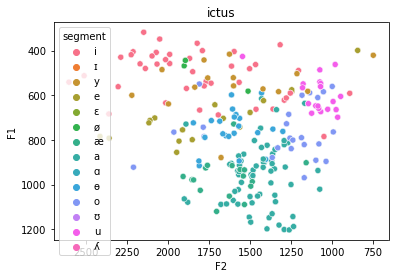
\includegraphics[width=0.9\linewidth]{figures/ictus}
%\caption{ictus}
%\label{ictus_space}
%\end{subfigure}
%\begin{subfigure}{0.5\textwidth}
%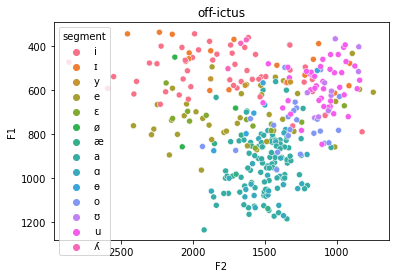
\includegraphics[width=0.9\linewidth]{figures/off-ictus}
%\caption{off-ictus}
%\label{offictus_space}
%\end{subfigure}
%\caption{ictus and off-ictus vowels}
%\label{ickoffVcharts}
%\end{figure}
%
%Looking at \ref{ickoffVcharts},  we do see a general trend of vowels in \ref{ictus_space} covering less area, with major categories a bit more diffuse compared to \ref{offictus_space}, where back vowels go much further back, and major vowel groups are clustered more closely. 
%
%\begin{table}[h]
%\caption{ordinary least squares, euc x stress}
%\begin{tabular}{lccccrr}
%\hline
%  &         coef   & std err    &      t    &  P>|t|    &  0.025   &   0.975  \\
%\hline
%Intercept    &   849.8434  &   24.962    & 34.045   &   0.000   &  800.820   &  898.866 \\
%stressed T.1  &  1.5645   &  33.485   &   0.047    &  0.963  &   -64.196    &  67.325 \\
%\hline
%\end{tabular}
%\label{ols_eucstress}
%\end{table}
%
%
%In \ref{ols_eucstress}, we see that as we expected, a stressed syllable correlates with an increase in euclidean distance, but this effect is not significant. It is interesting that at the word-level domain, the prominent position {\it does} have the larger space, vaguely apparent in \ref{stressunVcharts}. 
%
%
%\begin{figure}[h]
%\begin{subfigure}{0.5\textwidth}
%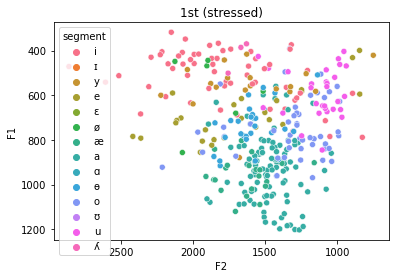
\includegraphics[width=0.9\linewidth]{figures/first}
%\caption{primary stress}
%\label{stress_space}
%\end{subfigure}
%\begin{subfigure}{0.5\textwidth}
%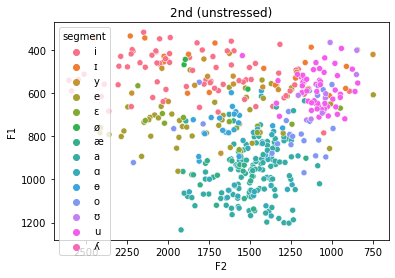
\includegraphics[width=0.9\linewidth]{figures/second}
%\caption{unstress}
%\label{unstress_space}
%\end{subfigure}
%\caption{(primary) stressed and unstressed vowels}
%\label{stressunVcharts}
%\end{figure}
%
%
%One wonders if the collapsing of strong and weak syllables in each other hierarchy is reducing the effect of prominence on vowel space: remember the asymmetry of conflict combinations in \ref{stressick}. To examine this, a linear regression is run once again, this time with both ictus and stress as categorical predictors for euclidean distance. 
%
%\begin{table}[h]
%\caption{ordinary least squares, euc x ictus+stress}
%\begin{centering}
%\begin{tabular}{lccccccr}
%\hline
%  &         coef   & std err    &      t    &  P>|t|    &  0.025   &   0.975  \\
%\hline
%Intercept        &    891.1615  &   28.178  &   31.627   &   0.000   &  835.824  &   946.499 \\
%T.ictus  	&	-104.6468  &   33.929   &  -3.084   &   0.002   & -171.279   &  -38.014 \\
%T.1         	&	0.0678   &  33.257   &   0.002    &  0.998   &  -65.244   &   65.380 \\
%\hline
%
%\end{tabular}
%\end{centering}
%\label{ols_eucboth}
%\end{table}
%
%In the resulting model \ref{ols_eucboth}, we once again see significant effects (p<0.05) of song prominence: that off-ictus has a larger vowel space, and ictus position has a smaller euclidean distance between F1 and F2, even when stress is included in the model. Stress still has a positive coefficient here, but the effect is still not significant. When we bring both factors into the model, we see the same pattern as before, but without any improvement to the model of ictus alone. 
%
%
%
%\begin{figure}[htbp]
%\begin{subfigure}{0.5\textwidth}
%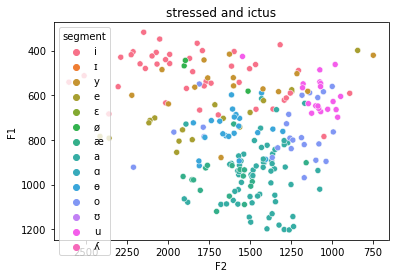
\includegraphics[width=0.9\linewidth]{figures/stressed-ictus.png}
%\caption{concord: stressed in ictus}
%\label{space_concord_ictus}
%\end{subfigure}
%\begin{subfigure}{0.5\textwidth}
%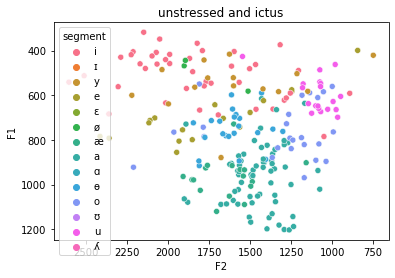
\includegraphics[width=0.9\linewidth]{figures/unstressed-ictus.png}
%\caption{conflict: unstressed in ictus}
%\label{conflict_unstrIck}
%\end{subfigure}
%\\
%\begin{subfigure}{0.5\textwidth}
%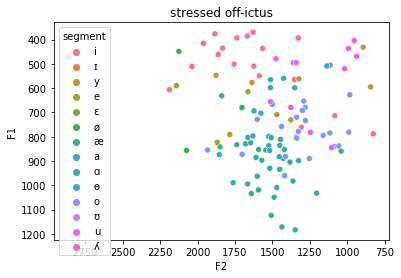
\includegraphics[width=0.9\linewidth]{figures/stressedoff-ictus.png}
%\caption{conflict: stressed in off-ictus}
%\label{conflict_str_off}
%\end{subfigure}
%\begin{subfigure}{0.5\textwidth}
%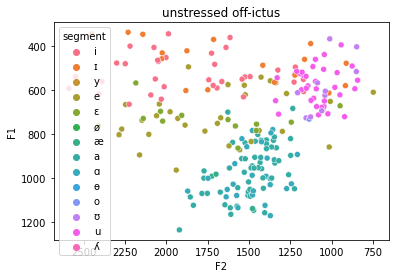
\includegraphics[width=0.9\linewidth]{figures/unstressedoff-ictus.png}
%\caption{concord: unstressed in ictus}
%\label{concord:unoff}
%\end{subfigure}
%
%\caption{Vowel charts in conflicting and concordant prominence positions}
%\label{Vcharts_conAll}
%\end{figure}
%
%Song-level prominence is a better predictor of vowel space than word-level prominence: interestingly, off-ictus positions have a larger and more peripheral vowel space (p<0.05). 
%
%\subsection{Vowel Duration} 
%Mean vowel duration for syllables in ictus position is slightly higher than those in off-ictus position, seen in Table \ref{ictusdur}
%
%
%\begin{table}[htb]
%\caption{ictus position and mean duration}
%\begin{center}
%\begin{tabular}{cc}
%& vowel duration \\
%\hline
%ictus  &   0.213561 \\
%off    &  0.198477 \\
%\end{tabular}
%\end{center}
%\label{ictusdur}
%\end{table}%
%
%In \ref{ickydur} we see significant effects of song-level metrical position and vowel duration. Ictus position has a positive slope of (p< 0.05). The effect is small: remember, though, that this ictus sample includes syllables that are both stressed and unstressed, and in all three quantities. In spite of weight and prominence variation at other levels of the prosodic hierarchy, vowel durations in ictus position are longer than those that fall in off-ictus positions. 
%
%\begin{table}[h]
%\caption{ordinary least squares, duration x ictus}
%\begin{center}
%\begin{tabular}{lcccccr}
%\hline
%    &    coef  &  std.err     &     t   &  P>|t|   &   [0.025     0.975] \\
% \hline	
%Intercept    &    0.2136   &   0.006 &    37.287  &    0.000     &  0.202      0.225 \\
%ictus[T.off]  &  -0.0151  &    0.007   &  -2.062      & 0.040    &  -0.029     -0.001 \\
%\hline
%\end{tabular}
%\end{center}
%\label{ickydur}
%\end{table}%
%
%In \ref{stressdur} are the mean durations of stressed and unstressed vowels. This level of vowel duration contrast is also preserved, and the difference between the two is greater than the ictus-off difference in \ref{ictusdur}. 
%
%\begin{table}[h]
%\caption{stress and mean duration}
%\begin{center}
%\begin{tabular}{cc}
%stress & mean duration \\ 
%\hline
%0   &  0.186972 \\
%1   &  0.218175 \\
%\end{tabular}
%\end{center}
%\label{stressdur}
%\end{table}%\\
%
%Looking at \ref{olsstress}, syllables that have primary word stress are a good predictor for an increase in vowel duration, seen by the positive coefficient. The effect is significant  (p < 0.05) but slight, with a tiny positive slope. 
%
%
%\begin{table}[h]
%\caption{ordinary least squares, duration x stress}
%\begin{center}
%\begin{tabular}{llcccr}
%\hline
%       &             coef &   std.err      &    t     & P>|t|   &   [0.025      0.975]	\\
%\hline
%Intercept    &     0.1870      & 0.005   &  35.412   &   0.000      & 0.177       0.197	\\
%stressed[T.1]  &   0.0312     & 0.007   &   4.406     & 0.000    &   0.017       0.045	\\
%\hline
%\end{tabular}
%\end{center}
%\label{olsstress}
%\end{table}%
%
%At this point, both levels of the prosodic hierarchy in these songs are preserving contrasts via vowel duration. Putting both song and word levels of the prosodic hierarchy for the model in \ref{sticky}, we get a slightly better model, with both stress and ictus position having significant effects on vowel duration. It appears that stress has a greater influence on vowel duration than ictus position does, though both correlate with an increase in vowel duration.
%\begin{table}[h]
%\caption{ordinary least squares, duration x stress+ictus}
%\begin{center}
%\begin{tabular}{lllllll}
%\hline
%                               &                     coef    &std.err  &        t    &  P>|t|   &   [0.025      0.975]	\\
%Intercept                             &            0.1808    &  0.006   &  30.221   &   0.000     &  0.169       0.193	\\
%stressed[T.1]                    &                 0.0314     & 0.007   &   4.450    &  0.000     &  0.018       0.045	\\
%ictus [T.ictus]    & 0.0156   &   0.007     & 2.159    &  0.031      & 0.001       0.030	\\
%\hline
%\end{tabular}
%\end{center}
%\label{sticky}
%\end{table}%
%\subsection{Conflict resolution between ictus and stress}
%
%These results illustrate a negotiation between the song and word level prominences. While both levels retained the cue of vowel duration, neither prominence position retained the vowel space pattern. However, we saw the assymmetry in that the off-ictus position was often the home of stressed syllables, and that this seemed to be a preference. There were more stressed than unstressed syllables in off-ictus. This suggests that vowel space is only a cue for prominence in the event of a conflict. The stressed syllable accomodates the preservation of ictus prominence, but as ictus is not using the cue of vowel space, this is available to the stressed syllables in weak positions in order to indicated their prominence at the word level. 
%
%\section{Syllable Quantity} 
%
%Now we look to see if the quantity contrast bears out in song. 
%\begin{table}[h]
%\caption{quantity and vowel duration}
%\begin{center}
%\begin{tabular}{cc}
%quantity  & duration \\
%1   & 0.208675 \\
%2   & 0.198997 \\
%3  &  0.210527 \\
%\end{tabular}
%\end{center}
%\label{qdur}
%\end{table}%
%
%Looking at the mean vowel durations for syllable quantities in \ref{qdur}, we see that vowel duration does not vary much across categories. This is surprising: we would expect to see vowel duration decrease as syllable quantity increases (to accomodate the additional vowels and coda consonants: remember that double vowels in Q2 and Q3 are cut in half and measured separately here). 
%
%
%
%
%\begin{table}[h]
%\caption{duration x quantity}
%\begin{center}
%\begin{tabular}{llccccr}
%\hline
%                &                coef  &  std.err     &     t   &   P>|t|   &   [0.025      0.975]	\\
%Intercept          &                0.1990  &    0.005   &  38.479  &    0.000    &   0.189       0.209		\\
%Quantity[T.1]  &   0.0097   &   0.008     & 1.251    &  0.211    &  -0.006       0.025	\\
%Quantity[T.3]   &  0.0115    &  0.011    &  1.055    &  0.292    &  -0.010       0.033	\\
%\hline
%\end{tabular}
%\end{center}
%\label{qdurols}
%\end{table}%
%
%
%
%
%Looking at the model  \ref{qdurols}, quantity category is not a significant predictor for vowel duration. This confirms the earlier findings of earlier studies of spoken and sung {\it regilaul}, \citep{}, where the duration contrast between syllable weights was lost in absolute duration but preserved in the ratios of first and second syllables in Q2 and Q3.  \\
%
%%
%%Bringing ictus status into the model  we see a significant (p< 0.05) positive slope for vowel durations in ictus position, in line with earlier analysis of ictus and vowel duration. Both Q1 an Q3 have a positive slope, but neither is significant. \\
%
%
%Now we look at the effects of stress and quantity. Since we know that stress is a significant predictor for vowel duration, adding it to this model may shed some light on the quantity contrast pattern. In \ref{stressqols} the intercept in this model is stressed syllables in Q2: as Q3 is always stressed, stress position is the only place where all three syllable quantities contrast. 
%We see that stressed Q1 syllables have a significant positive slope, with a coeff of 0.024 and a p < 0.05.  
%
%Q3 vowels have a negative slope, as we would expect but is not statistically significant. This means that in stressed position, vowel duration alone is not carrying the contrast between Q2 and Q3. 
%
%Unstressed Q2 vowels have a significant (p < 0.05) negative slope compared to the intercept, in line with our earlier results in stress and vowel duration. 
%
%This confirms the notion that the contrast between Q2 and Q3 is not on the strong first syllable of the foot alone: this lends support to the foot as the domain of this quantity contrast. \\
%
%\begin{table}[h]
%\caption{duration x quantity+stress}
%\begin{center}
%\begin{tabular}{llcccccr}
%\hline
%                                           &    coef    & std.err    &      t   &   P>|t|   &   [0.025      0.975]	\\
%                                           \hline
%Intercept                        &            0.2142   &   0.006    & 36.657  &    0.000    &   0.203       0.226	\\
%C(stressed,)[T.0]  &  -0.0417   &   0.008   &  -5.207  &    0.000   &   -0.057      -0.026	\\
%C(quantity, [T.1]     &0.0238    &  0.008  &    2.953    &  0.003       &0.008       0.040	\\
%C(quantity, )[T.3]    & -0.0036    &  0.011  &   -0.329    &  0.742     & -0.025       0.018	\\
%\hline
%\end{tabular}
%\end{center}
%\label{stressqols}
%\end{table}%
%
%In \ref{ickqols}, we see that while the ictus and off-ictus vowel duration contrast is preserved (p,0.05), neither Q1 nor Q3 has a vowel duration significantly different from Q2. 
%
%\begin{table}[h]
%\caption{duration x quantity+ictus}
%\begin{center}
%\begin{tabular}{llcccccr}
%\hline
%                                           &    coef    & std.err    &      t   &   P>|t|   &   [0.025     & 0.975]	\\
%                                           \hline
%Intercept                        &    0.2083     & 0.007   &  29.662   &   0.000    &   0.195    &   0.222 \\
%C(ictus, [T.off]  &  -0.0144 &      0.007    & -1.961 &     0.050   &   -0.029  &  2.08e-05 \\
%C(quantity[T.1]     &     0.0088  &    0.008     & 1.144     & 0.253      &-0.006     &  0.024 \\
%C(quantity)[T.3]       &   0.0101   &   0.011     &  0.921      & 0.357      &-0.011    &   0.032 \\
%       
%\hline
%\end{tabular}
%\end{center}
%\label{ickqols}
%\end{table}%
%
